% !TeX spellcheck = en_US
% !TeX root = 1315LectureNotes.tex
% !TeX encoding = UTF-8
\RequirePackage[l2tabu,orthodox]{nag}
\documentclass[oneside]{scrbook}
\usepackage{microtype}
\usepackage{fullpage}
\usepackage{mathtools}
\usepackage[bookmarks=true,breaklinks=true,linktoc=all,unicode=true,%
 hidelinks]{hyperref}
\usepackage{cleveref}
\usepackage{amssymb}
\usepackage{gensymb}
\usepackage{textcomp}
\usepackage{enumitem}
\usepackage[svgnames,table,hyperref]{xcolor}
\usepackage[framemethod=TikZ]{mdframed}
\usepackage{array}
\usepackage{tikz}
\usetikzlibrary{arrows}

\setcounter{secnumdepth}{0}
\setcounter{tocdepth}{3}

\providecommand{\reals}{\mathbb{R}}
\providecommand{\lt}{<}
\providecommand{\gt}{>}
\providecommand{\defeq}{\vcentcolon=}
\providecommand{\abs}[1]{\left| #1\right|}
\providecommand{\parens}[1]{\left( #1\right)}
\providecommand{\set}[1]{\left\{ #1\right\}}
\providecommand{\intervaloo}[2]{\left( #1, #2\right)}
\providecommand{\intervalco}[2]{\left[ #1, #2\right)}
\providecommand{\intervaloc}[2]{\left( #1, #2\right]}
\providecommand{\intervalcc}[2]{\left[ #1, #2\right]}
\providecommand{\fahrenheit}{\textdegree F}

% Color names come from Wikipedia article on "Web Colors", X11 section
% https://en.wikipedia.org/wiki/Web_colors#X11_color_names

% Environment colors are "White" colors
\colorlet{genericFrameColor}{Wheat} % brown/wheat
\colorlet{genericFrameBgColor}{Cornsilk} % brown/cornsilk
\colorlet{exampleColor}{PaleGreen} % green/pale green
\colorlet{procedureColor}{PaleTurquoise} % blue/pale turquoise
\colorlet{definitionColor}{MistyRose} % white/misty rose
\colorlet{theoremColor}{LavenderBlush} % white/lavender blush

% Text/Variable colors span the colors for colorblindness reasons
\colorlet{varColor}{CornflowerBlue}
\providecommand{\constcolor}[1]{\textcolor{varColor}{#1}}
\colorlet{varColor1}{Crimson} % red/crimson 
\colorlet{varColor2}{SpringGreen} % green/spring green
\colorlet{varColor3}{Yellow} % yellow/yellow

\mdfdefinestyle{basicFrameStyle}{
    outerlinewidth=2pt,
    innertopmargin=\baselineskip,
    frametitlefont=\sffamily\bfseries
}
\mdfdefinestyle{genericFrameStyle}{style=basicFrameStyle}
\mdfapptodefinestyle{genericFrameStyle}{
    linecolor=genericFrameColor,
    frametitlebackgroundcolor=genericFrameColor,
    backgroundcolor=genericFrameBgColor
}
\newmdenv[style=genericFrameStyle]{genericFrame}

\newcounter{example}[section]
\renewcommand{\theexample}{\arabic{chapter}-\arabic{example}}
\mdfdefinestyle{exampleStyle}{style=basicFrameStyle}
\mdfapptodefinestyle{exampleStyle}{
    linecolor=exampleColor,
    settings={\stepcounter{example}},
    frametitle={~Example~\theexample\hbox{~}},
    frametitlebackgroundcolor=exampleColor
}
\newmdenv[style=exampleStyle]{example}

\newcounter{procedure}[section]
\renewcommand{\theprocedure}{\arabic{chapter}-\arabic{procedure}}
\mdfdefinestyle{procedureStyle}{style=basicFrameStyle}
\mdfapptodefinestyle{procedureStyle}{
    linecolor=procedureColor,
    settings={\stepcounter{procedure}},
    frametitle={~Procedure~\theexample\hbox{~}},
    frametitlebackgroundcolor=procedureColor
}
\newmdenv[style=procedureStyle]{procedure}

\newcounter{definition}[section]
\renewcommand{\thedefinition}{\arabic{chapter}-\arabic{definition}}
\mdfdefinestyle{definitionStyle}{style=basicFrameStyle}
\mdfapptodefinestyle{definitionStyle}{
    linecolor=definitionColor,
    settings={\stepcounter{definition}},
    frametitle={~Definition~\theexample\hbox{~}},
    frametitlebackgroundcolor=definitionColor
}
\newmdenv[style=definitionStyle]{definition}

\newcounter{theorem}[section]
\renewcommand{\thetheorem}{\arabic{chapter}-\arabic{theorem}}
\mdfdefinestyle{theoremStyle}{style=basicFrameStyle}
\mdfapptodefinestyle{theoremStyle}{
    linecolor=theoremColor,
    settings={\stepcounter{theorem}},
    frametitle={~Theorem~\theexample\hbox{~}},
    frametitlebackgroundcolor=theoremColor
}
\newmdenv[style=theoremStyle]{theorem}


\begin{document}
\title{College Algebra Lecture Notes}
\subtitle{2016 Spring}
\author{Andrew Cousino}
\maketitle

\frontmatter
\tableofcontents
\listoffigures
\listoftables

\mainmatter
\part{Equations and Inequalities}
% !TeX encoding = UTF-8
% !TeX spellcheck = en_US
% !TeX root = 1315LectureNotes.tex
\chapter{Solutions Bound in Sets}\label{chap:numAndSets}
\begin{genericFrame}[frametitle={~New Things\hbox{~}}]
    \textbf{\Large\sffamily Definitions}
    \begin{description}[style=nextline]
        \item[Set] a collection of items
        \item[Element of set \(A\)] An item inside the set \(A\). If
         \(x\) is an element of the set \(A\), then we write
         \(x\in A\). Otherwise, we write \(x\notin A\) to say that the
         item \(x\) is not an element of \(A\).
        \item[Empty Set] the unique set which has nothing inside it,
         i.e. no elements. We write \(\emptyset\) to mean the empty 
         set.
        \item[Real Numbers] the set which contains all integers,
         fractions, and irrational numbers. We write \(\reals\) to
         mean the real numbers, or more properly, the set of real
         numbers.
    \end{description}
    \textbf{\Large\sffamily Notation}
    \begin{itemize}
        \item Roster Method for describing a set
        \item Set-Builder Method for describing a set
    \end{itemize}
\end{genericFrame}

\section{Sets Contain Solutions}
\subsection{Definition}\label{sec:set_defn}
A \textbf{set} is simply a container, albeit an abstract container, of 
various items. When we talk about a specific set, lets just use an 
arbitrary set \(A\) as an example, the items contained inside this set 
\(A\) are called the \textbf{elements} of this set. When talking about 
a specific item, say \(x\) for example, we will write \(x\in A\) to 
mean that the item \(x\) is an element of the set \(A\). Likewise, we 
write \(x\notin A\) to mean that \(x\) is not an element of \(A\).

\subsection{Naming Sets}
We need to have some examples of the kind of sets that we'll be working
with in this class. There are two ways of naming, or describing, a set.

\subsubsection{Roster Method}
Here is one such example.
\[\set{2, 3, 5, 7}\]
This is the set that contains the numbers 2, 3, 5, and 7, and no other
elements. The method of writing a set in this way is known as the
\textbf{roster method}. It's most convenient when dealing with sets 
that have a small number of elements.

\subsubsection{Set-Builder Method}
But we will be dealing with sets that have infinitely many members. For
these sets, we describe them using \textbf{Set-Builder method}.
\[\set{x\mid x\lt 5} \text{read: the set of all element \(x\) such %
    that \(x\) is less than 5}\]

It starts, and ends, with the same curly braces \(\set{}\), describes
the type of elements it contains, e.g. a single number represented by
\(x\), and gives a condition which determine whether or not an item is
a member in the set, e.g. \(x\lt 5\). For our set above, if any single
number, represented by \(x\), is less than 5, then \(x\) is an element
of this. And every element of our set must be numbers less than 5.
Another way to represent this set is with a number line.

\begin{center}
	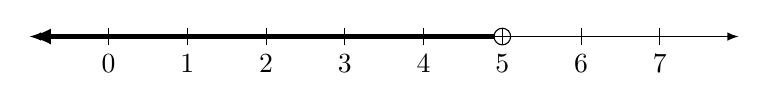
\begin{tikzpicture}
		\draw[latex-,ultra thick] (-1,0) -- (5, 0);
		\draw[fill=white] (5,0) circle (3pt);
		\draw[latex-latex] (-1,0) -- (8, 0);
		\foreach \x in {0, 1, 2, 3, 4, 5, 6, 7}
			\draw[shift={(\x,0)}] (0, 3pt) -- (0, -3pt);
		\foreach \x in {0, 1, 2, 3, 4, 5, 6, 7}
			\draw[shift={(\x,0)}] (0,-3pt) node[below] {\(\x\)};
	\end{tikzpicture}
\end{center}

\section{Sets in College Algebra}
The other common types of sets we will encounter are the set of all 
real numbers \(\mathbb{R}\), and the empty set \(\emptyset\), which is 
the set that contains nothing at all.
% !TeX encoding = UTF-8
% !TeX spellcheck = en_US
% !TeX root = 1315LectureNotes.tex
\chapter{Linear Equations and Inequalities}\label{chap:linearRatEqns}
\begin{genericFrame}[frametitle={~New Things\hbox{~}}]
    \textbf{\Large\sffamily Definitions}
    \begin{description}[style=nextline]
        \item[Linear Equation] An equation which can be put in the
         form \(\constcolor{a} x + \constcolor{b}=0\).
        \item[Contradiction] An equation or inequality which has no
         solution, like \(x + 1 = x\), or is outright
         false, like \(0=1\).
        \item[Identity] An equation or inequality which is true
         regardless of the value of the variable(s), for
         example \(\parens{x+1}^{2}-\parens{x-1}^{2}=4 x\).
        \item[Conditional] An equation or inequality which is true when
         the variables have certain values, and is false otherwise.
    \end{description}
    \textbf{\Large\sffamily Notations}
    \begin{description}[style=nextline]
    	\item[Interval Notation] A method of denoting an interval using
    	`\(\left(\right.\)', `\(\left[\right.\)', `\(\left.\right)\)',
    	and `\(\left.\right]\)' to indicate the inclusion
    	`\(\left[\right]\)' or exclusion `\(\left(\right)\)' of
    	endpoints. `\(\cup\)' is used to join together intervals when 
    	needed.
    \end{description}
\end{genericFrame}

\section{Linear Equations}
\subsection{Examples}
\begin{example}
	The cost, in dollars, to rent a storage unit for \(t\) months is
    given by \(C\defeq 150 + 52.50 t\). If you have \$1,200 budgeted 
    for storage, how long can you rent such a unit?
	
	\begin{description}
		\item[WANT] Time \(t\) when cost is \$1,200.
		\item[KNOW] \(C=\$1,200\).
	\end{description}
	\begin{align*}
		C & = 1200 \\
		150 + 52.50 t & = 1200 \\
		52.50 t & = 1050 \\
		t & = 20 \\
	\end{align*}
	So you can rent the unit for up to 20 months while staying within 
    budget.
\end{example}

\begin{example}
	How much of a 4\% acid solution should be mixed with 200 mL of a 
    12\% to make a 9\% solution?
	
	\begin{description}
		\item[WANT] Amount of 4\% solution, \(x\), to add.
	\end{description}
	\begin{center}
		\begin{tabular}{cccc}
			 & \textbf{4\% Solution} & \textbf{12\% Solution} & 
			 \textbf{9\% Solution} \\
			\textbf{Total Amount} & \(x\) & 200 & x + 200 \\
			\textbf{Amount of Acid} & \(0.04 x\) & \(0.12\cdot 200\) & 
             \(0.09\parens{x + 200}\) \\
		\end{tabular}
	\end{center}
	\begin{align*}
		0.04 x + 0.12\cdot 200 & = 0.09\parens{x + 200} \\
		0.04 x + 24 & = 0.09 x + 18 \\
		6 & = 0.05 x \\
		x & = 120 \\
	\end{align*}
	Mix 120 mL of 4\% solution with 200 mL of 12\% solution to get 320 
    mL of 9\%.
\end{example}

\begin{example}
	Two companies, company A and company B, both make yard signs among 
    other things. Company A charges \$1.20 per sign, while B charges a 
    flat fee of \$15.90 for the design on top of \$1.10 per sign. 
    First write out a model for the cost of ordering \(x\) signs from 
    both companies. Obviously, Company A is cheaper if you're only 
    going to make a few signs; but if you're going to make a lot of 
    signs then eventually Company B becomes cheaper. How many signs 
    need to be ordered so that the costs from both companies become 
    equal?
	
	\begin{align*}
		A & = 1.2 x \\
		B & = 1.1 x + 15.9 \\
	\end{align*}
	
	\begin{description}
		\item[WANT] Number of signs needed, \(x\), for \(A=B\).
	\end{description}
	\begin{align*}
		A & = B \\
		1.2 x & = 1.1 x + 15.9 \\
		0.1 x & = 15.9 \\
		x & = 159 \\
	\end{align*}
	
	So ordering up to 159 signs, company A is cheaper. But when ordering over 159 signs, company B is cheaper.
\end{example}

\subsection{Contradictions and Identities}
An equation involving the variable \(x\) that is true when \(x\) is one
value but false when \(x\) is another value is called a
\textbf{conditional equation}. There are equations which are true
regardless of what the value of \(x\) is. We call these kinds of 
equations \textbf{identities} or tautologies. Finally, the third type 
of equation is one which is never true for any value of \(x\). These 
are \textbf{contradictions}.

\begin{example}
    Identify each equation as either as being conditional, a 
    contradiction, or an identity. Also find the solution set of each.
    \begin{enumerate}
        \item \(4 x + 1 - x = 6 x - 2\)
        \item \(2\parens{-5 x - 1} = 2 x - 12 x + 6\)
        \item \(2\parens{3 x - 1} = 6\parens{x + 1} - 8\)
    \end{enumerate}
    
    \begin{enumerate}
        \item
            \begin{align*}
                4 x + 1 - x & = 6 x - 2 \\
                3 x + 1 & = 6 x - 2 \\
                3 & = 3 x \\
                1 & = x \\
                x & = 1 \\
            \end{align*}
            If \(x=1\), then the original equation will be true. So 
            this is a conditional equation whose solution set is
            \(\set{1}\).
        \item
            \begin{align*}
                2\parens{-5 x - 1} & = 2 x - 12 x + 6 \\
                -10 x - 2 & = -10 x + 6 \\
                0 & = 8 \\
            \end{align*}
            This is clearly false. So the original equation must always
            be false, regardless of the value of \(x\). This is a
            contraction whose solution set is the empty set 
            \(\emptyset\).
        \item
            \begin{align*}
                2\parens{3 x - 1} & = 6\parens{x + 1} - 8 \\
                6 x - 2 & = 6 x + 6 - 8 \\
                6 x - 2 & = 6 x - 2 \\
                0 & = 0 \\
            \end{align*}
            This is obviously true. The original equation must always 
            be true. So we have an identity with the solution set 
            being the set of all real numbers \(\reals\).
    \end{enumerate}
\end{example}

\section{Linear Inequalties}
\subsection{Interval Notation}
Most of the sets that we work with in this class will be written in a
style known as interval notations. As the name suggests, this notation
represents intervals on the number line. There are 9 basic types of
intervals which are listed in \cref{tab:int_notat} along with their
meaning.

\begin{table}[h]
	\centering
	\renewcommand{\arraystretch}{1.5}
	\def\myNumlineVOffset{-0.75\height}
	\newlength{\myRadius}
	\setlength{\myRadius}{2pt}
    \rowcolors{2}{WhiteSmoke}{GhostWhite}
	\begin{tabular}{>{\centering}m{5em}ccp{13.5em}}
	
		\textbf{Interval Notation} &
			\textbf{Set Notation} &
			\textbf{Number Line} &
			\textbf{Meaning} \\ \hline
		% (-\infty, b)
		\(\intervaloo{-\infty}{b}\) &
			\(\set{x\mid x\lt b}\) &
			\raisebox{\myNumlineVOffset}{
				\begin{tikzpicture}
					\draw[latex-,ultra thick] (0,0) -- (2,0);
					\draw[fill=white] (2,0) circle (\myRadius);
					\draw[latex-latex] (0,0) -- (3, 0);
					\foreach \x in {1, 2}
						\draw[shift={(\x,0)}] %
                         (0,\myRadius)--(0,-\myRadius);
					\node[above] at (2,0.5\myRadius) %
					 {\(\constcolor{b}\)};
				\end{tikzpicture}} &
			all \#s \(\lt b\)\\
		% (-\infty, b]
		\(\intervaloc{-\infty}{\textcolor{varColor}{b}}\) &
			\(\set{x\mid x\leq\constcolor{b}}\) &
			\raisebox{\myNumlineVOffset}{
				\begin{tikzpicture}
					\draw[latex-,ultra thick] (0,0) -- (2,0);
					\draw[fill=black] (2,0) circle (\myRadius);
					\draw[latex-latex] (0,0) -- (3, 0);
					\foreach \x in {1, 2}
						\draw[shift={(\x,0)}] %
                         (0,\myRadius)--(0,-\myRadius);
					\node[above] at (2,0.5\myRadius) %
					 {\(\constcolor{b}\)};
				\end{tikzpicture}} &
			all \#s \(\leq\textcolor{varColor}{b}\)\\
		% (a, b)
		\(\intervaloo{\constcolor{a}}{\constcolor{b}}\) &
			\(\set{x\mid \constcolor{a}\lt x\lt\constcolor{b}}\) &
			\raisebox{\myNumlineVOffset}{
				\begin{tikzpicture}
					\draw[-,ultra thick] (1,0) -- (2, 0);
					\draw[fill=white] (1,0) circle (\myRadius);
					\draw[fill=white] (2,0) circle (\myRadius);
					\draw[latex-latex] (0,0) -- (3, 0);
					\foreach \x in {1, 2}
						\draw[shift={(\x,0)}] %
                         (0,\myRadius)--(0,-\myRadius);
					\node[above] at (1,0.5\myRadius) %
					 {\(\constcolor{a}\)};
					\node[above] at (2,0.5\myRadius) %
					 {\(\constcolor{b}\)};
				\end{tikzpicture}} &
			all \#s btwn \(\constcolor{a}\) \& \(\constcolor{b}\), %
            excl. both endpoints\\
		% (a, b]
		\(\intervaloc{\textcolor{varColor}{a}}{%
            \textcolor{varColor}{b}}\) &
			\(\set{x\mid \constcolor{a}\lt x\leq\constcolor{b}}\) &
			\raisebox{\myNumlineVOffset}{
				\begin{tikzpicture}
					\draw[-,ultra thick] (1,0) -- (2, 0);
					\draw[fill=white] (1,0) circle (\myRadius);
					\draw[fill=black] (2,0) circle (\myRadius);
					\draw[latex-latex] (0,0) -- (3, 0);
					\foreach \x in {1, 2}
						\draw[shift={(\x,0)}] %
                         (0,\myRadius)--(0,-\myRadius);
					\node[above] at (1,0.5\myRadius) %
					 {\(\constcolor{a}\)};
					\node[above] at (2,0.5\myRadius) %
					 {\(\constcolor{b}\)};
				\end{tikzpicture}} &
			all \#s btwn \(\constcolor{a}\) \& \(\constcolor{b}\), %
            excl. \(\constcolor{a}\)\\
		% [a, b)
		\(\intervalco{\textcolor{varColor}{a}}{%
            \textcolor{varColor}{b}}\) &
			\(\set{x\mid \constcolor{a}\leq x\lt\constcolor{b}}\) &
%			\raisebox{\myNumlineVOffset}{
				\begin{tikzpicture}
					\draw[-,ultra thick] (1,0) -- (2, 0);
					\draw[fill=black] (1,0) circle (\myRadius);
					\draw[fill=white] (2,0) circle (\myRadius);
					\draw[latex-latex] (0,0) -- (3, 0);
					\foreach \x in {1, 2}
						\draw[shift={(\x,0)}] %
                         (0,\myRadius)--(0,-\myRadius);
					\node[above] at (1,0.5\myRadius) %
					 {\(\constcolor{a}\)};
					\node[above] at (2,0.5\myRadius) %
					 {\(\constcolor{b}\)};
				\end{tikzpicture} &
			all \#s btwn \(\constcolor{a}\) \& \(\constcolor{b}\) % 
            excl. \(\constcolor{b}\)\\
		% [a, b]
		\(\intervalcc{\textcolor{varColor}{a}}{%
            \textcolor{varColor}{b}}\) &
			\(\set{x\mid \constcolor{a}\leq x\leq\constcolor{b}}\) &
			\raisebox{\myNumlineVOffset}{
				\begin{tikzpicture}
					\draw[-,ultra thick] (1,0) -- (2, 0);
					\draw[fill=black] (1,0) circle (\myRadius);
					\draw[fill=black] (2,0) circle (\myRadius);
					\draw[latex-latex] (0,0) -- (3, 0);
					\foreach \x in {1, 2}
						\draw[shift={(\x,0)}] %
                         (0,\myRadius)--(0,-\myRadius);
					\node[above] at (1,0.5\myRadius) %
					 {\(\constcolor{a}\)};
					\node[above] at (2,0.5\myRadius) %
					 {\(\constcolor{b}\)};
				\end{tikzpicture}} &
			all \#s btwn \(\constcolor{a}\) \& %
            \(\constcolor{b}\)\\
		% [a, +\infty)
		\(\intervalco{\constcolor{a}}{+\infty}\) &
			\(\set{x\mid x\geq\constcolor{a}}\) &
			\raisebox{\myNumlineVOffset}{
		 		\begin{tikzpicture}
					\draw[-latex,ultra thick] (1,0) -- (3,0);
					\draw[fill=black] (1,0) circle (\myRadius);
					\draw[latex-latex] (0,0) -- (3, 0);
					\foreach \x in {1, 2}
						\draw[shift={(\x,0)}] %
                         (0,\myRadius)--(0,-\myRadius);
					\node[above] at (1,0.5\myRadius) %
					 {\(\constcolor{a}\)};
				\end{tikzpicture}} &
			all numbers \(\geq\constcolor{a}\) \\
		% (a, +\infty)
		\(\intervaloo{\constcolor{a}}{+\infty}\) &
			\(\set{x\mid x\gt\constcolor{a}}\) &
			\raisebox{\myNumlineVOffset}{
				\begin{tikzpicture}
					\draw[-latex,ultra thick] (1,0) -- (3,0);
					\draw[fill=white] (1,0) circle (\myRadius);
					\draw[latex-latex] (0,0) -- (3, 0);
					\foreach \x in {1, 2}
						\draw[shift={(\x,0)}] %
                         (0,\myRadius)--(0,-\myRadius);
					\node[above] at (1,0.5\myRadius) %
					 {\(\constcolor{a}\)};
				\end{tikzpicture}} &
			all numbers \(\gt\constcolor{a}\) \\
		% (-\infty, +\infty)
		\(\intervaloo{-\infty}{+\infty}\) &
			\(\reals\) &
			\raisebox{0.2\height}{
				\begin{tikzpicture}
					\draw[latex-latex,ultra thick] (0,0) -- (3,0);
					\foreach \x in {1, 2}
						\draw[shift={(\x,0)}] %
                         (0,\myRadius)--(0,-\myRadius);
				\end{tikzpicture}} &
			all real numbers\\
	\end{tabular}
	\caption{Table of Interval Notation}
    \label{tab:int_notat}
\end{table}

\subsection{Joining Intervals Together}
We will also want to join two intervals together. To join two 
intervals, say for example \(\intervalco{-1}{2}\) and 
\(\intervaloo{3}{+\infty}\), we write 
\(\intervalco{-1}{2}\cup\intervaloo{3}{+\infty}\).

\begin{center}
	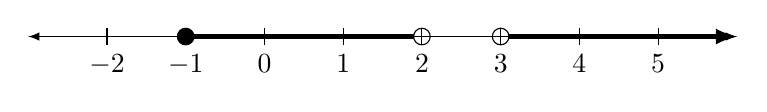
\begin{tikzpicture}
		\draw[-,ultra thick] (-1,0) -- (2, 0);
		\draw[-latex,ultra thick] (3, 0) -- (6, 0);
		\draw[fill=white] (2, 0) circle (3pt);
		\draw[fill=white] (3, 0) circle (3pt);
		\draw[fill=black] (-1, 0) circle (3pt);
		\draw[latex-latex] (-3,0)--(6,0);
		\foreach \x in {-2, -1, 0, 1, 2, 3, 4, 5}
			\draw[shift={(\x,0)}] (0, 3pt) -- (0, -3pt);
		\foreach \x in {-2, -1, 0, 1, 2, 3, 4, 5}
			\draw[shift={(\x,0)}] (0,-3pt) node[below] {\(\x\)};
	\end{tikzpicture}
\end{center}

\subsection{Examples of Linear Inequalities}
\begin{example}
	Donovan has offers for two different sales jobs. Job A pays a base 
	salary of \$25,000 plus 10\% commission on all sales. Job B pays a 
	base salary of \$30,000 plus 8\% commission. How much would 
	Donovan have to sell for the salary from Job A to exceed that of 
	Job B?
	
	\begin{align*}
		A & \defeq 25000 + 0.10 x \\
		B & \defeq 30000 + 0.08 x \\
		A & \gt B \\
		25000 + 0.10 x & \gt 30000 + 0.08 x \\
		0.02 x & \gt 5000 \\
		x & \gt 250000 \\
	\end{align*}
	So the solution set is the interval 
	\(\intervaloo{250,000}{+\infty}\). This means that Donovan must 
	sell at least \$250,000 in order for Job A to pay better than Job 
	B.
\end{example}

\begin{example}
	Body temperature usually between 36.5\,\celsius and 
	37.5\,\celsius. Given that \(C=\frac{5}{9} \parens{F - 32}\) 
	converts from
	\(F\)\,\fahrenheit to \(C\)\,\celsius, find the typical range for 
	body temperature in \fahrenheit.
	
	\begin{gather}
		36.5 \lt C \lt 37.5 \\
		36.5 \lt \frac{5}{9}\parens{F - 32} \lt 37.5 \\
		4.5 \lt \frac{5}{9} F - \frac{160}{9} \lt 5.5 \\
		\frac{977}{18} \lt \frac{5}{9} F \lt \frac{995}{18} \\
		\frac{977}{10} \lt F \lt \frac{199}{2} \\
		97.7 \lt F \lt 99.5 \\
	\end{gather}
	
	In Fahrenheit, typical body temperature ranges between 
	97.5--99.5\,\fahrenheit.
\end{example}

\begin{example}
	For what values of \(x\) will the following expressions avoid 
	taking square roots of negative numbers.
	
	\begin{enumerate}
		\item \(\sqrt{x-6}\)
		\item \(\sqrt{6-x}\)
	\end{enumerate}
	
	\begin{enumerate}
		\item \begin{align*}
			x - 6 & \geq 0 \\
			x & \geq 6 \\
		\end{align*}
		The values of \(x\) that avoid square roots of negative 
		numbers are the values of the interval 
		\(\intervalco{6}{+\infty}\).
		
		\item \begin{align*}
			6 - x & \geq 0 \\
			6 & \geq x \\
			x & \leq 6 \\
		\end{align*}
		The desired values of \(x\) are exactly those in the interval 
		\(\intervaloc{-\infty}{6}\).
	\end{enumerate}
\end{example}

\begin{example}
	Solve the following inequalities.
	\begin{enumerate}
		\item \(3\parens{2 x + 1} + 4\leq 6 x + 2\)
		\item \(9 + 4 c\gt 3\parens{c + 1} + c\)
	\end{enumerate}
	
	\begin{enumerate}
		\item \begin{align*}
			3\parens{2 x + 1} + 4 & \leq 6 x + 2 \\
			6 x + 3 + 4 & \leq 6 x + 2 \\
			7 & \leq 2 \\
		\end{align*}
		This is a contradiction. So the original inequality is a 
		contradiction and has no solution. The solution set is empty 
		\(\emptyset\).
		
		\item \begin{align*}
			9 + 4 c & \gt 3\parens{c + 1} + c \\
			9 + 4 c & \gt 3 c + 3 + c \\
			9 + 4 c & \gt 4 c + 3 \\
			6 & \gt 0 \\
		\end{align*}
		This is always true. So the original inequality is an identity 
		and every \(x\)-value is a solution. The solution set is all 
		reals \(\reals\).
	\end{enumerate}
\end{example}
% !TeX encoding = UTF-8
% !TeX spellcheck = en_US
% !TeX root = 1315LectureNotes.tex
\chapter{Complex Numbers}
% !TeX encoding = UTF-8
% !TeX spellcheck = en_US
% !TeX root = 1315LectureNotes.tex
\chapter{Quadratic Equations}\label{chap:quadEqns}
\begin{genericFrame}[frametitle={~New Things\hbox{~}}]
    \textbf{\Large\sffamily Definitions}
    \begin{description}[style=nextline]
        \item[Quadratic Equation] An equation which can be put in the %
        form \(\constcolor{a} x^{2} + \constcolor{b} x + %
         \constcolor{c}=0\).
    \end{description}

    \noindent\textbf{\Large\sffamily Procedures}
    \begin{description}[style=nextline]
    	\item[Factoring a Quadratic]
        \item[Completing the Square] A process that allows us to %
         rewrite a quadratic from standard form into vertex form.
        \item[Quadratic Formula]
    \end{description}

	\noindent\textbf{\Large\sffamily Notation}
	\begin{description}
		\item[Standard Form of a Quadratic] \(\constcolor{a} x^{2} +
		 \constcolor{b} x + \constcolor{c}\)
		\item[Vertex Form of a Quadratic] \(\constcolor{a}
		 \parens{x - \constcolor{h}}^{2} + \constcolor{k}\)
	
	\end{description}
\end{genericFrame}
\section{Factoring}
\section{Completing the Square}
\section{Quadratic Formula}

% !TeX encoding = UTF-8
% !TeX spellcheck = en_US
% !TeX root = 1315LectureNotes.tex
\chapter{Polynomial and Rational Equations}
\begin{genericFrame}[frametitle={~New Things\hbox{~}}]
    \textbf{\Large\sffamily Definitions}
    \begin{description}[style=nextline]
    	\item[Polynomial Expression]
    	\item[Polynomial Equation]
    	\item[Rational Expression]
    	\item[Rational Equation]
    \end{description}

    \noindent\textbf{\Large\sffamily Procedures}
    \begin{description}[style=nextline]
    	\item[Factoring a Polynomial]
        \item[Solving a Rational Equation]
    \end{description}
\end{genericFrame}
% !TeX encoding = UTF-8
% !TeX spellcheck = en_US
% !TeX root = 1315LectureNotes.tex
\chapter{Polynomial and Rational Inequalities}\label{chap:PolyRatIneq}
\begin{genericFrame}[frametitle={~Important Things\hbox{~}}]
    \textbf{\Large\sffamily Definitions}
    \begin{description}[style=nextline]
        \item[Polynomial Expression]
        \item[Rational Expression]
        \item[Partition Numbers]
        \item[Polynomial Inequality]
        \item[Rational Inequalities]
    \end{description}
\end{genericFrame}


\part{Functions and Relations}
\chapter{Graphs and Circles}
\chapter{Functions and Their Graphs}
\chapter{Transformations of Functions}
\chapter{Arithmetic of Functions}
\chapter{Inverse Functions}

\part{Library of Functions}
\chapter{Linear Functions}
\chapter{Quadratic Functions}
\chapter{Polynomial Functions}
\chapter{Dividing Polynomials}
\chapter{Zeros of Polynomial Functions}
\chapter{Rational Functions}
\chapter{Exponential Functions}
\chapter{Logarithmic Functions}

\part{Linear Systems}
\chapter{System of Linear Equations}
\chapter{Introduction to Matrices}
\chapter{Inconsistent and Dependent Systems}
\chapter{Arithmetic with Matrices}
\chapter{Inverse Matrices and Matrix Equations}

%\backmatter
%\printglossary[style=index]
%\printsymbols
%\printindex
\end{document}